% 图 74.8 —— 由 `checks/emit_hand.py` 自动拼出（probe 精测 + prims2 图元分解）
%%
% ⚠ 这是**稿子不是成品**：跑 `checks/checkhand.py 74.8` 看指标 + 看叠合图。
%%
%% ⚠ 待核：
%   · 本图 probe 报出阴影族 2 个 —— **本脚本不生成阴影**（要照原书手写）；prims2 的 strokes 里可能含阴影线，核对时留意别画重
%   · 可疑字形 2 项（空心圈 ⊙ 常被认成字母 o）—— 见文件末
%%
\documentclass[12pt]{standalone}
\usepackage{fontspec}
\setsansfont{Arial}
\newfontfamily\mfallback{DejaVu Sans}
\usepackage{tikz}
\begin{document}
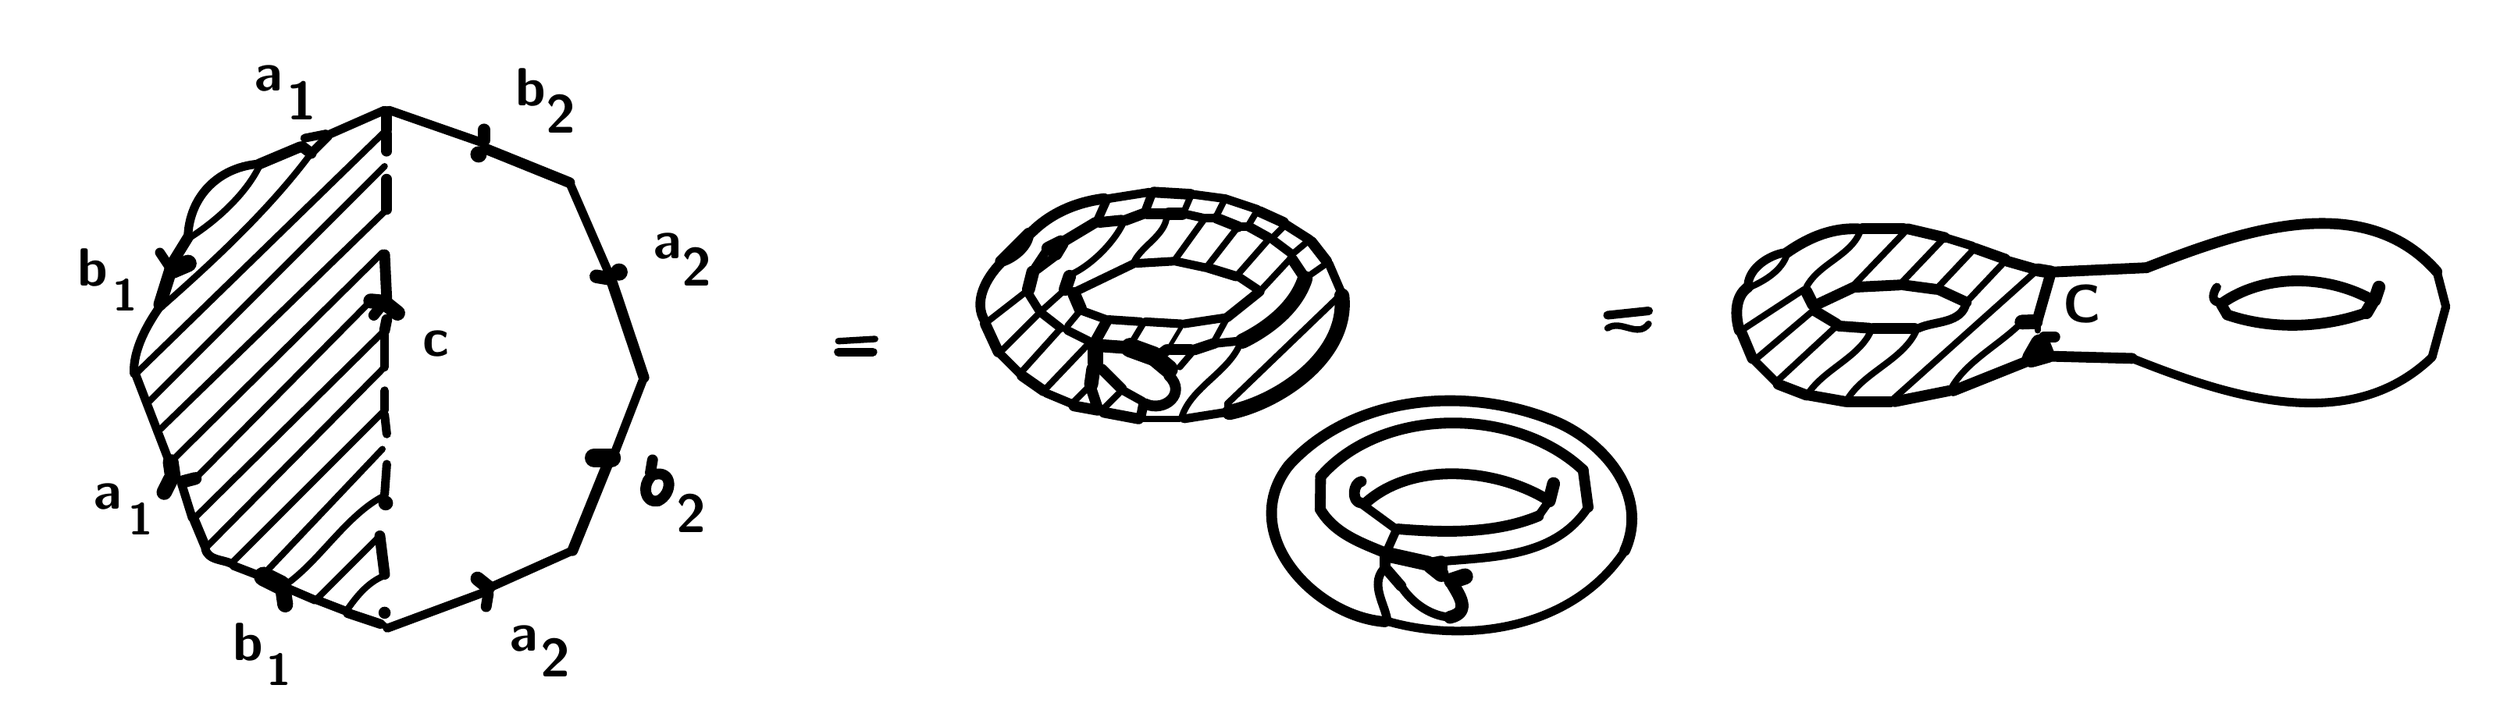
\begin{tikzpicture}[x=1pt, y=-1pt, line width=8.7pt, line cap=round, line join=round]

  %% ════ 填充区（prims2 的 fills）════

  %% ════ 直线段（prims2 的 strokes）════
  \draw[line width=8.7pt] (265.0,202.0) -- (273.0,202.0);
  \draw[line width=4.0pt] (168.0,41.0) -- (143.0,52.0);
  \draw[line width=3.0pt] (563.0,117.0) -- (577.0,101.0);
  \draw[line width=5.3pt] (652.0,251.0) -- (657.0,250.0);
  \draw[line width=4.0pt] (142.0,53.0) -- (134.0,61.0);
  \draw[line width=4.0pt] (537.0,140.0) -- (520.0,139.0);
  \draw[line width=4.0pt] (611.0,126.0) -- (605.0,112.0);
  \draw[line width=3.0pt] (571.0,89.0) -- (568.0,94.0);
  \draw[line width=3.0pt] (487.0,176.0) -- (494.0,169.0);
  \draw[line width=3.0pt] (501.0,179.0) -- (508.0,172.0);
  \draw[line width=5.0pt] (604.0,111.0) -- (597.0,102.0);
  \draw[line width=5.0pt] (826.0,173.0) -- (813.0,168.0);
  \draw[line width=5.0pt] (857.0,142.0) -- (876.0,142.0);
  \draw[line width=5.5pt] (829.0,131.0) -- (826.0,125.0);
  \draw[line width=5.5pt] (214.0,55.0) -- (214.0,50.0);
  \draw[line width=4.0pt] (471.0,134.0) -- (466.0,126.0);
  \draw[line width=5.0pt] (918.0,110.0) -- (904.0,105.0);
  \draw[line width=3.0pt] (933.0,143.0) -- (933.0,140.0);
  \draw[line width=5.0pt] (594.0,119.0) -- (588.0,110.0);
  \draw[line width=3.0pt] (594.0,119.0) -- (604.0,112.0);
  \draw[line width=5.2pt] (526.0,155.0) -- (530.0,152.0);
  \draw[line width=6.5pt] (495.0,168.0) -- (496.0,161.0);
  \draw[line width=6.0pt] (485.0,118.0) -- (483.0,124.0);
  \draw[line width=5.0pt] (452.0,153.0) -- (446.0,140.0);
  \draw[line width=4.0pt] (474.0,172.0) -- (486.0,177.0);
  \draw[line width=3.0pt] (574.0,124.0) -- (587.0,110.0);
  \draw[line width=4.0pt] (453.0,154.0) -- (462.0,163.0);
  \draw[line width=7.0pt] (174.0,135.0) -- (169.0,131.0);
  \draw[line width=5.0pt] (869.0,122.0) -- (849.0,123.0);
  \draw[line width=7.0pt] (651.0,251.0) -- (633.0,247.0);
  \draw[line width=5.7pt] (938.0,154.0) -- (936.0,149.0);
  \draw[line width=3.0pt] (395.0,147.0) -- (378.0,148.0);
  \draw[line width=4.0pt] (470.0,115.0) -- (478.0,109.0);
  \draw[line width=5.0pt] (939.0,155.0) -- (976.8,156.0);
  \draw[line width=4.0pt] (1115.6,155.4) -- (1122.0,132.0);
  \draw[line width=4.0pt] (1122.0,132.0) -- (1117.8,115.8);
  \draw[line width=5.0pt] (983.4,114.0) -- (940.0,116.0);
  \draw[line width=3.0pt] (553.0,90.0) -- (557.0,82.0);
  \draw[line width=8.0pt] (70.0,115.0) -- (77.0,112.0);
  \draw[line width=5.0pt] (871.0,96.0) -- (852.0,96.0);
  \draw[line width=5.0pt] (892.0,171.0) -- (867.0,176.0);
  \draw[line width=5.0pt] (509.0,170.0) -- (500.0,161.0);
  \draw[line width=5.0pt] (939.0,117.0) -- (933.0,138.0);
  \draw[line width=3.0pt] (813.0,166.0) -- (840.0,141.0);
  \draw[line width=5.0pt] (845.0,176.0) -- (865.0,176.0);
  \draw[line width=4.0pt] (510.0,171.0) -- (519.0,176.0);
  \draw[line width=3.0pt] (825.0,124.0) -- (796.0,143.0);
  \draw[line width=9.0pt] (513.0,151.0) -- (524.0,155.0);
  \draw[line width=4.0pt] (168.0,180.0) -- (168.0,171.0);
  \draw[line width=4.0pt] (538.0,89.0) -- (547.0,91.0);
  \draw[line width=6.0pt] (709.0,214.0) -- (707.0,222.0);
  \draw[line width=2.0pt] (531.0,151.0) -- (537.0,141.0);
  \draw[line width=4.0pt] (168.0,219.0) -- (169.0,205.0);
  \draw[line width=5.0pt] (77.0,100.0) -- (69.0,113.0);
  \draw[line width=4.0pt] (488.0,125.0) -- (515.0,112.0);
  \draw[line width=5.0pt] (215.0,271.0) -- (216.0,265.0);
  \draw[line width=6.0pt] (64.0,131.0) -- (69.0,115.0);
  \draw[line width=4.0pt] (469.0,114.0) -- (475.0,105.0);
  \draw[line width=3.0pt] (829.0,134.0) -- (803.0,156.0);
  \draw[line width=5.0pt] (495.0,170.0) -- (498.0,179.0);
  \draw[line width=4.0pt] (136.0,268.0) -- (122.0,262.0);
  \draw[line width=5.0pt] (167.0,131.0) -- (163.0,136.0);
  \draw[line width=5.0pt] (272.0,203.0) -- (255.0,245.0);
  \draw[line width=4.0pt] (255.0,245.0) -- (217.0,262.0);
  \draw[line width=3.0pt] (866.0,175.0) -- (933.0,115.0);
  \draw[line width=5.9pt] (75.0,213.0) -- (80.4,211.6);
  \draw[line width=3.0pt] (80.4,211.6) -- (161.6,129.4);
  \draw[line width=6.9pt] (161.6,129.4) -- (168.0,130.0);
  \draw[line width=4.0pt] (494.0,148.0) -- (484.0,143.0);
  \draw[line width=5.0pt] (168.0,143.0) -- (169.0,138.0);
  \draw[line width=5.0pt] (638.4,261.4) -- (632.0,254.0);
  \draw[line width=4.0pt] (503.0,82.0) -- (522.0,79.0);
  \draw[line width=4.0pt] (587.0,107.0) -- (579.0,101.0);
  \draw[line width=6.0pt] (481.0,102.0) -- (475.0,105.0);
  \draw[line width=5.0pt] (482.0,103.0) -- (479.0,108.0);
  \draw[line width=5.0pt] (473.0,171.0) -- (463.0,164.0);
  \draw[line width=5.0pt] (502.0,139.0) -- (497.0,148.0);
  \draw[line width=4.0pt] (702.0,229.0) -- (707.0,222.0);
  \draw[line width=3.0pt] (558.0,180.0) -- (558.0,177.0);
  \draw[line width=3.0pt] (558.0,177.0) -- (610.0,127.0);
  \draw[line width=5.0pt] (844.0,176.0) -- (827.0,173.0);
  \draw[line width=3.0pt] (519.0,184.0) -- (536.0,184.0);
  \draw[line width=5.0pt] (552.0,149.0) -- (543.0,152.0);
  \draw[line width=5.0pt] (519.0,89.0) -- (511.0,92.0);
  \draw[line width=6.0pt] (512.0,151.0) -- (498.0,150.0);
  \draw[line width=6.0pt] (537.0,89.0) -- (531.0,89.0);
  \draw[line width=3.0pt] (917.0,112.0) -- (900.0,130.0);
  \draw[line width=3.0pt] (579.0,100.0) -- (584.0,95.0);
  \draw[line width=5.0pt] (169.0,50.0) -- (169.0,42.0);
  \draw[line width=4.0pt] (63.0,190.0) -- (58.0,177.0);
  \draw[line width=3.0pt] (63.0,190.0) -- (168.0,88.0);
  \draw[line width=4.0pt] (63.0,190.0) -- (68.0,203.0);
  \draw[line width=4.0pt] (168.0,145.0) -- (168.0,160.0);
  \draw[line width=3.0pt] (168.0,160.0) -- (86.0,243.0);
  \draw[line width=5.0pt] (453.0,111.0) -- (466.0,98.0);
  \draw[line width=5.0pt] (886.0,124.0) -- (871.0,122.0);
  \draw[line width=5.0pt] (573.0,88.0) -- (584.0,93.0);
  \draw[line width=5.0pt] (631.0,253.0) -- (631.0,248.0);
  \draw[line width=3.0pt] (482.0,125.0) -- (472.0,134.0);
  \draw[line width=5.0pt] (941.0,146.0) -- (936.0,146.0);
  \draw[line width=7.0pt] (497.0,158.0) -- (497.0,151.0);
  \draw[line width=9.0pt] (112.0,257.0) -- (120.0,261.0);
  \draw[line width=4.0pt] (734.0,136.0) -- (753.0,134.0);
  \draw[line width=6.5pt] (211.0,258.0) -- (216.0,262.0);
  \draw[line width=6.3pt] (272.0,119.0) -- (266.0,118.0);
  \draw[line width=4.0pt] (802.0,157.0) -- (812.0,167.0);
  \draw[line width=4.0pt] (563.0,118.0) -- (572.0,124.0);
  \draw[line width=4.0pt] (903.0,104.0) -- (890.0,100.0);
  \draw[line width=4.0pt] (533.0,111.0) -- (516.0,112.0);
  \draw[line width=3.0pt] (547.0,92.0) -- (534.0,110.0);
  \draw[line width=3.0pt] (872.0,97.0) -- (848.0,122.0);
  \draw[line width=5.0pt] (919.0,111.0) -- (933.0,115.0);
  \draw[line width=4.0pt] (658.0,255.0) -- (658.0,251.0);
  \draw[line width=3.0pt] (167.0,107.0) -- (70.0,203.0);
  \draw[line width=7.1pt] (652.0,252.0) -- (657.0,256.0);
  \draw[line width=5.0pt] (291.0,209.0) -- (292.0,203.0);
  \draw[line width=5.0pt] (1018.0,131.0) -- (1020.8,135.8);
  \draw[line width=6.0pt] (1085.2,134.8) -- (1088.0,130.0);
  \draw[line width=4.0pt] (111.0,257.0) -- (98.0,252.0);
  \draw[line width=5.0pt] (497.0,93.0) -- (482.0,102.0);
  \draw[line width=3.0pt] (541.0,81.0) -- (538.0,88.0);
  \draw[line width=3.0pt] (870.0,121.0) -- (890.0,100.0);
  \draw[line width=4.0pt] (558.0,137.0) -- (538.0,140.0);
  \draw[line width=4.5pt] (558.0,137.0) -- (573.0,125.0);
  \draw[line width=3.0pt] (558.0,137.0) -- (552.0,148.0);
  \draw[line width=5.0pt] (517.0,184.0) -- (501.0,181.0);
  \draw[line width=4.5pt] (562.0,118.0) -- (549.0,114.0);
  \draw[line width=4.0pt] (563.0,148.0) -- (553.0,149.0);
  \draw[line width=3.0pt] (471.0,135.0) -- (453.0,153.0);
  \draw[line width=8.4pt] (930.0,156.0) -- (934.0,149.0);
  \draw[line width=3.0pt] (489.0,135.0) -- (484.0,141.0);
  \draw[line width=3.0pt] (80.0,230.0) -- (167.0,144.0);
  \draw[line width=4.0pt] (394.0,153.0) -- (378.0,153.0);
  \draw[line width=3.0pt] (474.0,170.0) -- (494.0,149.0);
  \draw[line width=6.0pt] (1089.0,129.0) -- (1091.0,123.0);
  \draw[line width=6.0pt] (931.0,157.0) -- (938.0,155.0);
  \draw[line width=3.0pt] (595.0,102.0) -- (589.0,107.0);
  \draw[line width=3.0pt] (536.0,160.0) -- (542.0,153.0);
  \draw[line width=3.0pt] (53.0,163.0) -- (168.0,51.0);
  \draw[line width=4.5pt] (80.0,231.0) -- (85.0,243.0);
  \draw[line width=3.0pt] (137.0,267.0) -- (165.8,238.2);
  \draw[line width=5.0pt] (165.8,238.2) -- (168.0,256.0);
  \draw[line width=6.0pt] (466.0,124.0) -- (468.0,116.0);
  \draw[line width=5.1pt] (130.0,58.0) -- (134.0,61.0);
  \draw[line width=8.4pt] (525.0,156.0) -- (531.0,161.0);
  \draw[line width=5.0pt] (900.0,130.0) -- (887.0,124.0);
  \draw[line width=7.3pt] (70.0,211.0) -- (69.0,204.0);
  \draw[line width=3.0pt] (887.0,123.0) -- (903.0,106.0);
  \draw[line width=5.0pt] (509.0,92.0) -- (499.0,93.0);
  \draw[line width=5.0pt] (532.0,152.0) -- (541.0,152.0);
  \draw[line width=4.0pt] (58.0,177.0) -- (53.0,164.0);
  \draw[line width=3.0pt] (58.0,177.0) -- (168.0,67.0);
  \draw[line width=4.2pt] (475.0,105.0) -- (478.0,108.0);
  \draw[line width=4.0pt] (79.0,230.0) -- (74.0,214.0);
  \draw[line width=5.0pt] (215.0,59.0) -- (253.6,74.6);
  \draw[line width=4.0pt] (253.6,74.6) -- (272.0,117.0);
  \draw[line width=5.0pt] (725.0,224.9) -- (722.7,207.7);
  \draw[line width=5.0pt] (601.2,210.8) -- (601.0,225.9);
  \draw[line width=5.0pt] (890.0,100.0) -- (873.0,96.0);
  \draw[line width=7.3pt] (121.0,263.0) -- (122.0,270.0);
  \draw[line width=4.0pt] (557.0,82.0) -- (542.0,80.0);
  \draw[line width=4.0pt] (557.0,82.0) -- (572.0,87.0);
  \draw[line width=5.0pt] (129.0,58.0) -- (110.0,66.0);
  \draw[line width=5.0pt] (855.0,142.0) -- (841.0,141.0);
  \draw[line width=5.0pt] (553.0,91.0) -- (563.0,95.0);
  \draw[line width=4.0pt] (215.0,264.0) -- (169.2,281.0);
  \draw[line width=3.0pt] (169.2,281.0) -- (167.0,279.0);
  \draw[line width=4.0pt] (503.0,138.0) -- (518.0,139.0);
  \draw[line width=4.0pt] (520.0,88.0) -- (523.0,80.0);
  \draw[line width=4.0pt] (170.0,41.0) -- (213.0,56.0);
  \draw[line width=3.0pt] (549.0,113.0) -- (563.0,95.0);
  \draw[line width=3.0pt] (167.0,181.0) -- (98.0,250.0);
  \draw[line width=4.0pt] (548.0,91.0) -- (552.0,91.0);
  \draw[line width=6.0pt] (487.0,126.0) -- (490.0,133.0);
  \draw[line width=5.0pt] (831.0,131.0) -- (848.0,123.0);
  \draw[line width=5.0pt] (273.0,120.0) -- (288.0,164.8);
  \draw[line width=4.0pt] (288.0,164.8) -- (274.0,201.0);
  \draw[line width=5.0pt] (169.0,60.0) -- (169.0,52.0);
  \draw[line width=5.0pt] (524.0,79.0) -- (541.0,80.0);
  \draw[line width=4.0pt] (636.0,235.0) -- (621.0,224.0);
  \draw[line width=5.0pt] (168.0,108.0) -- (169.0,129.0);
  \draw[line width=4.0pt] (557.0,181.0) -- (538.0,184.0);
  \draw[line width=6.8pt] (925.8,139.2) -- (932.0,139.0);
  \draw[line width=7.1pt] (66.0,218.0) -- (69.0,212.0);
  \draw[line width=5.0pt] (894.0,171.0) -- (929.0,157.0);
  \draw[line width=4.5pt] (64.0,107.0) -- (68.0,113.0);
  \draw[line width=5.0pt] (169.0,73.0) -- (169.0,87.0);
  \draw[line width=4.0pt] (502.0,83.0) -- (498.0,92.0);
  \draw[line width=4.5pt] (166.0,279.0) -- (151.0,274.0);
  \draw[line width=4.5pt] (519.0,178.0) -- (518.0,183.0);
  \draw[line width=4.0pt] (141.0,52.0) -- (131.0,54.0);
  \draw[line width=7.5pt] (668.0,257.0) -- (662.0,259.0);
  \draw[line width=3.0pt] (519.0,140.0) -- (513.0,150.0);
  \draw[line width=4.5pt] (577.0,100.0) -- (568.0,95.0);
  \draw[line width=5.0pt] (487.0,178.0) -- (498.0,180.0);
  \draw[line width=6.0pt] (939.0,116.0) -- (933.0,115.0);
  \draw[line width=5.0pt] (521.0,89.0) -- (529.0,89.0);
  \draw[line width=4.0pt] (169.0,191.0) -- (168.0,182.0);
  \draw[line width=5.0pt] (830.0,134.0) -- (840.0,140.0);
  \draw[line width=4.0pt] (137.0,268.0) -- (150.0,273.0);
  \draw[line width=3.0pt] (167.0,198.0) -- (112.0,256.0);
  \draw[line width=3.8pt] (658.0,257.0) -- (661.0,259.0);
  \draw[line width=4.5pt] (585.0,94.0) -- (596.0,101.0);
  \draw[line width=3.0pt] (465.0,125.0) -- (447.0,139.0);
  \draw[line width=4.0pt] (563.0,95.0) -- (567.0,95.0);
  \draw[line width=4.0pt] (491.0,134.0) -- (502.0,138.0);
  \draw[line width=4.0pt] (534.0,111.0) -- (548.0,114.0);
  \draw[line width=5.0pt] (796.0,144.0) -- (801.0,156.0);
  \draw[line width=4.0pt] (481.0,142.0) -- (472.0,135.0);
  \draw[line width=3.0pt] (481.0,142.0) -- (463.0,162.0);
  \draw[line width=4.0pt] (636.0,236.0) -- (632.0,245.0);

  %% ════ 曲线（prims2 的 curves —— 三段式，坐标同为 (y,x)）════
  \draw[line width=4.5pt] (446.0,139.0) .. controls (440.2,129.9) and (446.4,118.8) .. (453.0,112.0);
  \draw[line width=3.0pt] (78.0,100.0) .. controls (90.1,92.3) and (103.8,79.9) .. (110.0,67.0);
  \draw[line width=5.0pt] (620.0,213.0) .. controls (616.2,213.7) and (615.3,222.5) .. (620.0,223.0);
  \draw[line width=7.0pt] (594.0,119.0) .. controls (589.8,132.1) and (577.2,142.0) .. (565.0,148.0);
  \draw[line width=4.0pt] (1017.0,130.0) .. controls (1012.9,129.7) and (1014.4,125.1) .. (1016.0,123.0);
  \draw[line width=4.0pt] (976.8,156.0) .. controls (1019.5,172.9) and (1076.9,192.8) .. (1115.6,155.4);
  \draw[line width=5.0pt] (1117.8,115.8) .. controls (1082.8,76.0) and (1023.4,98.5) .. (983.4,114.0);
  \draw[line width=3.0pt] (467.0,99.0) .. controls (466.1,105.1) and (459.5,110.2) .. (454.0,112.0);
  \draw[line width=4.0pt] (85.0,244.0) .. controls (86.1,249.6) and (92.8,249.0) .. (97.0,251.0);
  \draw[line width=3.0pt] (817.0,108.0) .. controls (814.6,115.3) and (806.9,120.0) .. (800.0,123.0);
  \draw[line width=3.0pt] (530.0,90.0) .. controls (529.5,98.8) and (518.7,103.6) .. (515.0,111.0);
  \draw[line width=7.0pt] (559.0,181.0) .. controls (582.9,176.0) and (614.1,154.2) .. (611.0,127.0);
  \draw[line width=6.0pt] (662.0,260.0) .. controls (664.9,265.2) and (671.3,273.4) .. (661.1,275.9);
  \draw[line width=4.0pt] (661.1,275.9) .. controls (652.0,275.3) and (643.5,269.3) .. (638.4,261.4);
  \draw[line width=5.0pt] (520.0,177.0) .. controls (529.1,181.2) and (539.4,172.1) .. (531.0,164.0);
  \draw[line width=5.0pt] (637.0,235.0) .. controls (658.9,236.8) and (682.3,237.2) .. (702.0,229.0);
  \draw[line width=3.0pt] (827.0,172.0) .. controls (834.7,160.8) and (850.8,155.2) .. (856.0,143.0);
  \draw[line width=5.0pt] (622.0,223.0) .. controls (644.0,203.2) and (683.3,207.0) .. (707.0,222.0);
  \draw[line width=5.0pt] (292.0,210.0) .. controls (301.7,206.9) and (301.5,218.9) .. (294.6,222.0);
  \draw[line width=5.0pt] (294.6,222.0) .. controls (288.0,223.2) and (287.4,214.6) .. (291.0,211.0);
  \draw[line width=5.0pt] (799.0,123.0) .. controls (792.7,127.4) and (793.1,136.6) .. (795.0,143.0);
  \draw[line width=3.0pt] (564.0,149.0) .. controls (558.9,162.2) and (541.3,169.4) .. (537.0,183.0);
  \draw[line width=5.0pt] (501.0,82.0) .. controls (488.4,83.6) and (476.3,88.5) .. (467.0,98.0);
  \draw[line width=5.0pt] (1020.8,135.8) .. controls (1041.1,142.8) and (1065.1,142.0) .. (1085.2,134.8);
  \draw[line width=3.0pt] (510.0,93.0) .. controls (505.6,102.3) and (495.3,112.6) .. (486.0,117.0);
  \draw[line width=3.0pt] (65.0,132.0) .. controls (89.1,110.8) and (115.0,86.6) .. (134.0,61.0);
  \draw[line width=4.0pt] (900.0,130.0) .. controls (898.2,140.0) and (885.3,138.6) .. (878.0,142.0);
  \draw[line width=5.0pt] (1088.0,129.0) .. controls (1067.5,117.4) and (1038.9,116.5) .. (1019.0,130.0);
  \draw[line width=5.0pt] (631.0,278.0) .. controls (598.1,275.5) and (562.1,236.8) .. (586.5,205.5);
  \draw[line width=5.0pt] (586.5,205.5) .. controls (616.2,172.9) and (667.8,168.9) .. (707.1,184.1);
  \draw[line width=5.0pt] (707.1,184.1) .. controls (731.0,192.9) and (753.9,218.5) .. (742.0,245.0);
  \draw[line width=4.0pt] (742.0,245.0) .. controls (718.9,280.1) and (671.4,288.6) .. (633.0,278.0);
  \draw[line width=4.0pt] (658.0,250.0) .. controls (682.1,247.9) and (710.0,247.8) .. (725.0,224.9);
  \draw[line width=5.0pt] (722.7,207.7) .. controls (691.4,178.2) and (629.5,178.1) .. (601.2,210.8);
  \draw[line width=5.0pt] (601.0,225.9) .. controls (607.6,237.1) and (619.9,241.4) .. (631.0,246.0);
  \draw[line width=3.0pt] (734.0,142.0) .. controls (740.3,137.8) and (748.0,146.8) .. (753.0,140.0);
  \draw[line width=3.0pt] (167.0,257.0) .. controls (160.2,260.0) and (155.2,266.0) .. (151.0,272.0);
  \draw[line width=3.0pt] (851.0,97.0) .. controls (846.7,108.5) and (831.8,112.0) .. (826.0,123.0);
  \draw[line width=3.0pt] (893.0,170.0) .. controls (899.9,157.3) and (915.4,149.8) .. (925.8,139.2);
  \draw[line width=3.0pt] (122.0,261.0) .. controls (137.9,249.9) and (149.9,229.2) .. (167.0,220.0);
  \draw[line width=5.0pt] (850.0,96.0) .. controls (837.6,95.5) and (826.9,100.1) .. (817.0,107.0);
  \draw[line width=4.0pt] (632.0,277.0) .. controls (630.8,269.8) and (624.5,261.0) .. (630.0,254.0);
  \draw[line width=3.0pt] (845.0,175.0) .. controls (852.6,162.3) and (870.9,156.7) .. (877.0,143.0);
  \draw[line width=4.0pt] (77.0,99.0) .. controls (78.0,80.7) and (91.1,67.8) .. (109.0,66.0);
  \draw[line width=4.0pt] (52.0,163.0) .. controls (51.5,152.5) and (57.7,140.9) .. (64.0,132.0);
  \draw[line width=4.0pt] (816.0,107.0) .. controls (808.8,108.1) and (799.5,114.1) .. (799.0,122.0);

  %% ════ 实心点 ════
  \fill (168.0,273.8) circle (2.8);
  \fill (211.5,61.5) circle (3.8);
  \fill (276.5,116.0) circle (4.0);
  \fill (168.5,223.0) circle (3.4);

  %% ════ 标签（probe 直接给的 \node 行）════
  %% ⚠ 全部补了 fill=white：文字在最上层，否则与曲线交叉干扰
     \node[anchor=center,inner sep=0pt,fill=white,font=\fontsize{30.0}{37.6}\selectfont] at (114.5,26.5) {\textsf{\textbf{\textit{a}}}};   % box(106,17,15,16)
     \node[anchor=center,inner sep=0pt,fill=white,font=\fontsize{30.0}{37.5}\selectfont] at (235.8,30.2) {\textsf{\textbf{\textit{b}}}};   % box(226,18,17,22)
     \node[anchor=center,inner sep=0pt,fill=white,font=\fontsize{23.0}{28.7}\selectfont] at (129.7,36.9) {\textsf{\textbf{1}}};   % box(123,29,8,15)
     \node[anchor=center,inner sep=0pt,fill=white,font=\fontsize{24.7}{30.9}\selectfont] at (249.6,42.9) {\textsf{\textbf{2}}};   % box(243,34,12,17)
     \node[anchor=center,inner sep=0pt,fill=white,font=\fontsize{32.0}{40.0}\selectfont] at (299.1,104.1) {\textsf{\textbf{\textit{a}}}};   % box(290,94,16,17)
     \node[anchor=center,inner sep=0pt,fill=white,font=\fontsize{30.7}{38.3}\selectfont] at (32.8,113.8) {\textsf{\textbf{\textit{b}}}};   % box(23,101,17,23)
     \node[anchor=center,inner sep=0pt,fill=white,font=\fontsize{24.7}{30.9}\selectfont] at (312.6,113.9) {\textsf{\textbf{2}}};   % box(306,105,12,17)
     \node[anchor=center,inner sep=0pt,fill=white,font=\fontsize{21.5}{26.9}\selectfont] at (48.0,126.9) {\textsf{\textbf{1}}};   % box(42,119,7,15)
     \node[anchor=center,inner sep=0pt,fill=white,font=\fontsize{24.2}{30.3}\selectfont] at (953.6,130.7) {\textsf{\textbf{\textit{C}}}};   % box(945,122,16,17)
     \node[anchor=center,inner sep=0pt,fill=white,font=\fontsize{31.4}{39.3}\selectfont] at (191.8,149.1) {\textsf{\textbf{\textit{c}}}};   % box(183,139,16,17)
     \node[anchor=center,inner sep=0pt,fill=white,font=\fontsize{32.0}{40.0}\selectfont] at (40.1,220.1) {\textsf{\textbf{\textit{a}}}};   % box(31,210,16,17)
     \node[anchor=center,inner sep=0pt,fill=white,font=\fontsize{23.6}{29.6}\selectfont] at (310.1,227.9) {\textsf{\textbf{2}}};   % box(304,219,11,17)
     \node[anchor=center,inner sep=0pt,fill=white,font=\fontsize{22.2}{27.8}\selectfont] at (55.1,230.4) {\textsf{\textbf{1}}};   % box(49,222,7,16)
     \node[anchor=center,inner sep=0pt,fill=white,font=\fontsize{30.0}{37.5}\selectfont] at (104.8,287.2) {\textsf{\textbf{\textit{b}}}};   % box(95,275,17,22)
     \node[anchor=center,inner sep=0pt,fill=white,font=\fontsize{31.0}{38.7}\selectfont] at (232.5,286.0) {\textsf{\textbf{\textit{a}}}};   % box(224,276,15,17)
     \node[anchor=center,inner sep=0pt,fill=white,font=\fontsize{23.6}{29.6}\selectfont] at (247.1,294.9) {\textsf{\textbf{2}}};   % box(241,286,11,17)
     \node[anchor=center,inner sep=0pt,fill=white,font=\fontsize{22.2}{27.8}\selectfont] at (119.1,300.4) {\textsf{\textbf{1}}};   % box(113,292,7,16)

  % 钉死画布：否则超出的图元/控制点会把页面撑大，1:1 回比就失准
  \pgfresetboundingbox
  \path[use as bounding box] (0,0) rectangle (1137,315);
\end{tikzpicture}
\end{document}

% ⚠ 待核清单（probe 拿不准，人眼过一遍）：
%   · 未识别/跳过：⑤ 跳过/未识别的字形
%   · 未识别/跳过：box(1013,119,82,25)
